\documentclass[11pt]{article}
\usepackage[utf8]{inputenc}
\usepackage{amsmath, amssymb}
\usepackage[margin=1in]{geometry}
\usepackage{tikz}

\begin{document}

\begin{center}
\textbf{STAT 410 -- Homework \#02}\\
Sections 2.1--2.3: Joint Distributions\\
Due: February 6, 2026\\[6pt]
By Tianyi Li
\end{center}

\bigskip

\textbf{3.} Let the joint p.d.f. for $(X, Y)$ be $f(x,y) = Cxy$, $0 < x < 2$, $0 < y < 2 + x$, zero otherwise.

\medskip

(a) Sketch of the support of $(X, Y)$:

\begin{center}
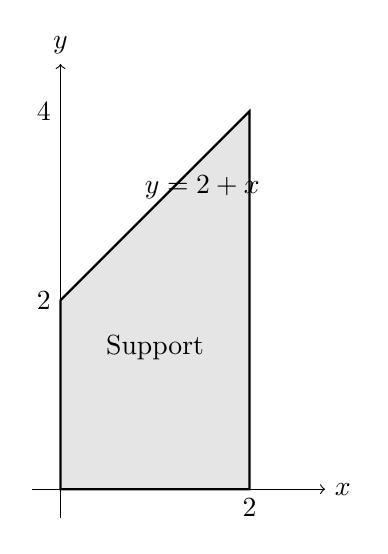
\begin{tikzpicture}[scale=1.2]
\draw[->] (-0.3,0) -- (2.8,0) node[right] {$x$};
\draw[->] (0,-0.3) -- (0,4.5) node[above] {$y$};
\draw[thick, fill=gray!20] (0,0) -- (2,0) -- (2,4) -- (0,2) -- cycle;
\draw[dashed] (0,2) -- (2,4);
\node at (1,1.5) {Support};
\node[below] at (2,0) {$2$};
\node[left] at (0,2) {$2$};
\node[left] at (0,4) {$4$};
\node at (1.5,3.2) {$y = 2 + x$};
\end{tikzpicture}
\end{center}

The support is the region $\{(x,y): 0 < x < 2, 0 < y < 2 + x\}$.

\medskip

(b) For a valid joint p.d.f., $\iint f(x,y)\, dA = 1$.
\[
\int_0^2 \int_0^{2+x} Cxy\, dy\, dx = 1
\]
Inner integral:
\[
\int_0^{2+x} Cxy\, dy = Cx \cdot \frac{y^2}{2}\Big|_0^{2+x} = \frac{Cx(2+x)^2}{2}
\]
Outer integral:
\[
\int_0^2 \frac{Cx(2+x)^2}{2}\, dx = \frac{C}{2} \int_0^2 x(4 + 4x + x^2)\, dx = \frac{C}{2} \int_0^2 (4x + 4x^2 + x^3)\, dx
\]
\[
= \frac{C}{2} \left[ 2x^2 + \frac{4x^3}{3} + \frac{x^4}{4} \right]_0^2 = \frac{C}{2} \left[ 8 + \frac{32}{3} + 4 \right] = \frac{C}{2} \cdot \frac{24 + 32 + 12}{3} = \frac{C}{2} \cdot \frac{68}{3} = \frac{34C}{3}
\]
Setting $\frac{34C}{3} = 1$, we get $\boxed{C = \frac{3}{34}}$.

\medskip

(c) The marginal p.d.f. of $X$ is:
\[
f_X(x) = \int_0^{2+x} \frac{3}{34}xy\, dy = \frac{3x}{34} \cdot \frac{y^2}{2}\Big|_0^{2+x} = \frac{3x(2+x)^2}{68}
\]
\[
\boxed{f_X(x) = \begin{cases} \frac{3x(2+x)^2}{68} & 0 < x < 2 \\ 0 & \text{otherwise} \end{cases}}
\]

\medskip

(d) For the marginal p.d.f. of $Y$, we need to find the range of $x$ for each $y$.

From $0 < y < 2 + x$ and $0 < x < 2$:
\begin{itemize}
\item If $0 < y \leq 2$: $x$ ranges from $0$ to $2$ (since $y < 2 + x$ is satisfied for all $x > 0$)
\item If $2 < y < 4$: $x$ ranges from $y - 2$ to $2$ (since we need $y < 2 + x \Rightarrow x > y - 2$)
\end{itemize}

For $0 < y \leq 2$:
\[
f_Y(y) = \int_0^2 \frac{3}{34}xy\, dx = \frac{3y}{34} \cdot \frac{x^2}{2}\Big|_0^2 = \frac{3y}{34} \cdot 2 = \frac{6y}{34} = \frac{3y}{17}
\]

For $2 < y < 4$:
\[
f_Y(y) = \int_{y-2}^2 \frac{3}{34}xy\, dx = \frac{3y}{34} \cdot \frac{x^2}{2}\Big|_{y-2}^2 = \frac{3y}{68}\left[4 - (y-2)^2\right]
\]
\[
= \frac{3y}{68}\left[4 - y^2 + 4y - 4\right] = \frac{3y}{68}(4y - y^2) = \frac{3y^2(4 - y)}{68}
\]

\[
\boxed{f_Y(y) = \begin{cases} \frac{3y}{17} & 0 < y \leq 2 \\[6pt] \frac{3y^2(4-y)}{68} & 2 < y < 4 \\[6pt] 0 & \text{otherwise} \end{cases}}
\]

\medskip

(e) $P(X + Y \leq 1.8)$:

The line $x + y = 1.8$ intersects the support. Since $0 < x < 2$ and $0 < y < 2 + x$, and the line $y = 1.8 - x$ intersects $y = 0$ at $x = 1.8$.

For $0 < x < 1.8$, $y$ ranges from $0$ to $\min(2+x, 1.8-x) = 1.8 - x$ (since $1.8 - x < 2 + x$ for $x > -0.1$).
\[
P(X + Y \leq 1.8) = \int_0^{1.8} \int_0^{1.8-x} \frac{3}{34}xy\, dy\, dx
\]
\[
= \frac{3}{34} \int_0^{1.8} x \cdot \frac{(1.8-x)^2}{2}\, dx = \frac{3}{68} \int_0^{1.8} x(1.8-x)^2\, dx
\]
Let $u = 1.8 - x$, or expand directly:
\[
= \frac{3}{68} \int_0^{1.8} x(3.24 - 3.6x + x^2)\, dx = \frac{3}{68} \int_0^{1.8} (3.24x - 3.6x^2 + x^3)\, dx
\]
\[
= \frac{3}{68} \left[ 1.62x^2 - 1.2x^3 + \frac{x^4}{4} \right]_0^{1.8}
\]
\[
= \frac{3}{68} \left[ 1.62(3.24) - 1.2(5.832) + \frac{10.4976}{4} \right]
\]
\[
= \frac{3}{68} \left[ 5.2488 - 6.9984 + 2.6244 \right] = \frac{3}{68}(0.8748) = \frac{2.6244}{68} \approx 0.0386
\]

$\boxed{P(X + Y \leq 1.8) \approx 0.0386}$

\medskip

(f) $P(X + Y \leq 3.0)$:

The line $x + y = 3$ intersects the boundary $y = 2 + x$ at $x + 2 + x = 3 \Rightarrow x = 0.5$.

We split the region:
\begin{itemize}
\item For $0 < x < 0.5$: $y$ from $0$ to $2 + x$ (entire strip below line)
\item For $0.5 \leq x < 2$: $y$ from $0$ to $3 - x$
\end{itemize}

\[
P(X + Y \leq 3) = \int_0^{0.5} \int_0^{2+x} \frac{3xy}{34}\, dy\, dx + \int_{0.5}^{2} \int_0^{3-x} \frac{3xy}{34}\, dy\, dx
\]

First integral (using result from part b pattern):
\[
\int_0^{0.5} \frac{3x(2+x)^2}{68}\, dx = \frac{3}{68} \int_0^{0.5} x(4 + 4x + x^2)\, dx
\]
\[
= \frac{3}{68}\left[2x^2 + \frac{4x^3}{3} + \frac{x^4}{4}\right]_0^{0.5} = \frac{3}{68}\left[0.5 + \frac{0.5}{3} + \frac{0.0625}{4}\right] = \frac{3}{68}(0.6823) \approx 0.0301
\]

Second integral:
\[
\int_{0.5}^{2} \frac{3x(3-x)^2}{68}\, dx = \frac{3}{68} \int_{0.5}^{2} x(9 - 6x + x^2)\, dx
\]
\[
= \frac{3}{68}\left[\frac{9x^2}{2} - 2x^3 + \frac{x^4}{4}\right]_{0.5}^{2}
\]
At $x = 2$: $18 - 16 + 4 = 6$. At $x = 0.5$: $1.125 - 0.25 + 0.0156 = 0.8906$.
\[
= \frac{3}{68}(6 - 0.8906) = \frac{3}{68}(5.1094) \approx 0.2254
\]

$\boxed{P(X + Y \leq 3.0) \approx 0.0301 + 0.2254 = 0.2555}$

\medskip

(g) $P(XY \leq 3.0)$:

The curve $xy = 3$ gives $y = 3/x$. This intersects:
\begin{itemize}
\item $y = 2 + x$ when $3/x = 2 + x \Rightarrow 3 = 2x + x^2 \Rightarrow x^2 + 2x - 3 = 0 \Rightarrow x = 1$
\item At $x = 1$: $y = 3$
\end{itemize}

For $0 < x < 1$: entire strip (since $xy < 3$ for $y < 2 + x \leq 3$ and $x < 1$)

For $1 \leq x < 2$: $y$ from $0$ to $\min(2+x, 3/x) = 3/x$

\[
P(XY \leq 3) = \int_0^{1} \int_0^{2+x} \frac{3xy}{34}\, dy\, dx + \int_{1}^{2} \int_0^{3/x} \frac{3xy}{34}\, dy\, dx
\]

First integral (from part b pattern, limit 0 to 1):
\[
= \frac{3}{68}\left[2x^2 + \frac{4x^3}{3} + \frac{x^4}{4}\right]_0^{1} = \frac{3}{68}\left[2 + \frac{4}{3} + \frac{1}{4}\right] = \frac{3}{68} \cdot \frac{43}{12} = \frac{43}{272} \approx 0.1581
\]

Second integral:
\[
\int_{1}^{2} \frac{3x}{34} \cdot \frac{(3/x)^2}{2}\, dx = \int_{1}^{2} \frac{3x}{34} \cdot \frac{9}{2x^2}\, dx = \int_{1}^{2} \frac{27}{68x}\, dx = \frac{27}{68}\ln x\Big|_1^2 = \frac{27\ln 2}{68} \approx 0.2752
\]

$\boxed{P(XY \leq 3.0) \approx 0.1581 + 0.2752 = 0.4333}$

\medskip

(h) $P(Y/X \leq 1.8)$:

The line $y = 1.8x$ intersects $y = 2 + x$ at $1.8x = 2 + x \Rightarrow 0.8x = 2 \Rightarrow x = 2.5 > 2$.

So within the support ($0 < x < 2$), the line $y = 1.8x$ is always below $y = 2 + x$.

At $x = 2$: $y = 1.8(2) = 3.6 < 4 = 2 + 2$. Good.

\[
P(Y/X \leq 1.8) = \int_0^{2} \int_0^{1.8x} \frac{3xy}{34}\, dy\, dx = \frac{3}{34} \int_0^{2} x \cdot \frac{(1.8x)^2}{2}\, dx
\]
\[
= \frac{3}{34} \int_0^{2} \frac{3.24x^3}{2}\, dx = \frac{3 \cdot 3.24}{68} \cdot \frac{x^4}{4}\Big|_0^2 = \frac{9.72}{68} \cdot 4 = \frac{38.88}{68} \approx 0.5718
\]

$\boxed{P(Y/X \leq 1.8) \approx 0.5718}$

\medskip

(i) $P(Y/X \leq 3.0)$:

The line $y = 3x$ intersects $y = 2 + x$ at $3x = 2 + x \Rightarrow 2x = 2 \Rightarrow x = 1$.

For $0 < x < 1$: $y$ from $0$ to $\min(2+x, 3x) = 3x$ (since $3x < 2 + x$ when $x < 1$)

For $1 \leq x < 2$: $y$ from $0$ to $2 + x$ (entire strip)

\[
P(Y/X \leq 3) = \int_0^{1} \int_0^{3x} \frac{3xy}{34}\, dy\, dx + \int_{1}^{2} \int_0^{2+x} \frac{3xy}{34}\, dy\, dx
\]

First integral:
\[
= \frac{3}{34} \int_0^{1} x \cdot \frac{9x^2}{2}\, dx = \frac{27}{68} \cdot \frac{x^4}{4}\Big|_0^1 = \frac{27}{272} \approx 0.0993
\]

Second integral (from part b pattern, limits 1 to 2):
\[
= \frac{3}{68}\left[2x^2 + \frac{4x^3}{3} + \frac{x^4}{4}\right]_1^{2} = \frac{3}{68}\left[\left(8 + \frac{32}{3} + 4\right) - \left(2 + \frac{4}{3} + \frac{1}{4}\right)\right]
\]
\[
= \frac{3}{68}\left[\frac{68}{3} - \frac{43}{12}\right] = \frac{3}{68} \cdot \frac{272 - 43}{12} = \frac{3}{68} \cdot \frac{229}{12} = \frac{229}{272} \approx 0.8419
\]

$\boxed{P(Y/X \leq 3.0) \approx 0.0993 + 0.8419 = 0.9412}$

\medskip

(j) For $X$ and $Y$ to be independent, we need $f(x,y) = f_X(x) \cdot f_Y(y)$ for all $(x,y)$.

The support of $(X,Y)$ is $\{0 < x < 2, 0 < y < 2 + x\}$, which is \textbf{not} a rectangle.

Since the support depends on both $x$ and $y$ together (the upper bound on $y$ depends on $x$), the joint distribution cannot factor into a product of marginals.

Alternatively, from parts (c) and (d):
\[
f_X(x) \cdot f_Y(y) = \frac{3x(2+x)^2}{68} \cdot \frac{3y}{17} = \frac{9xy(2+x)^2}{1156} \neq \frac{3xy}{34} = f(x,y)
\]

$\boxed{\text{No, } X \text{ and } Y \text{ are not independent.}}$

\end{document}
